Most change-point detection algorithms are not intended for usage in distributed mode. Experimentally obtained results show that algorithm used in single-node mode can really slow the stream processing graph.

\begin{figure}[h]
    \centering
    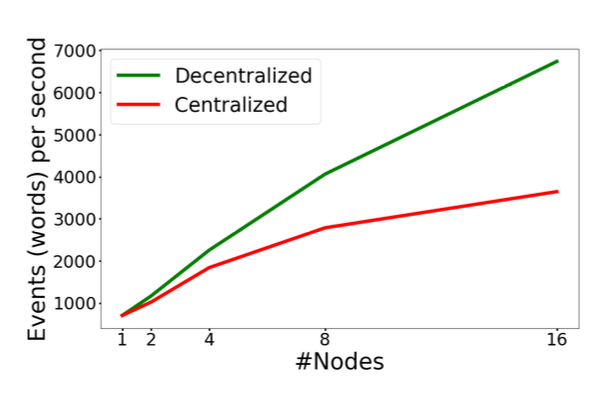
\includegraphics[scale=0.7]{throughput.png}
\end{figure}

``Decentralized'' line depicts throughput of system with distributed algorithm of change-detection while ``Centralized'' corresponds to throughput of system with single-node algorithm.

Thus, development an efficient distributed change-point detection algorithm is a practically important problem.